\section{Feature Characteristics}

\subsection{Feature Distribution Analysis}

Understanding the distribution of features within our dataset is critical for identifying potential preprocessing steps and informing model selection.

\subsubsection{Methodology:}

We utilized histograms to examine the distributions of pre-computed audio features across the dataset. This visualization aids in identifying features with non-normal distributions, which could potentially skew the performance of many machine learning algorithms that assume normally distributed data.

\subsubsection{Findings:}

\begin{itemize}
    \item \textbf{Skewed Distributions}: Certain features, especially those related to frequency and energy, exhibited skewed distributions. This skewness indicates that some preprocessing, such as log transformation or normalization, might be necessary to align these features more closely with a normal distribution.
    \item \textbf{Normal Distributions}: Mel-scaled energies, MFCCs, Centroid, Bandwidth, and Contrasts follow a normal distribution. These features capture aspects like frequency perception, sound "center of mass", frequency spread, and the difference between peak and valley energies in spectral bands, reflecting the tonal and noise characteristics of the sound.
\end{itemize}

\begin{figure}[!ht]
	\centering
	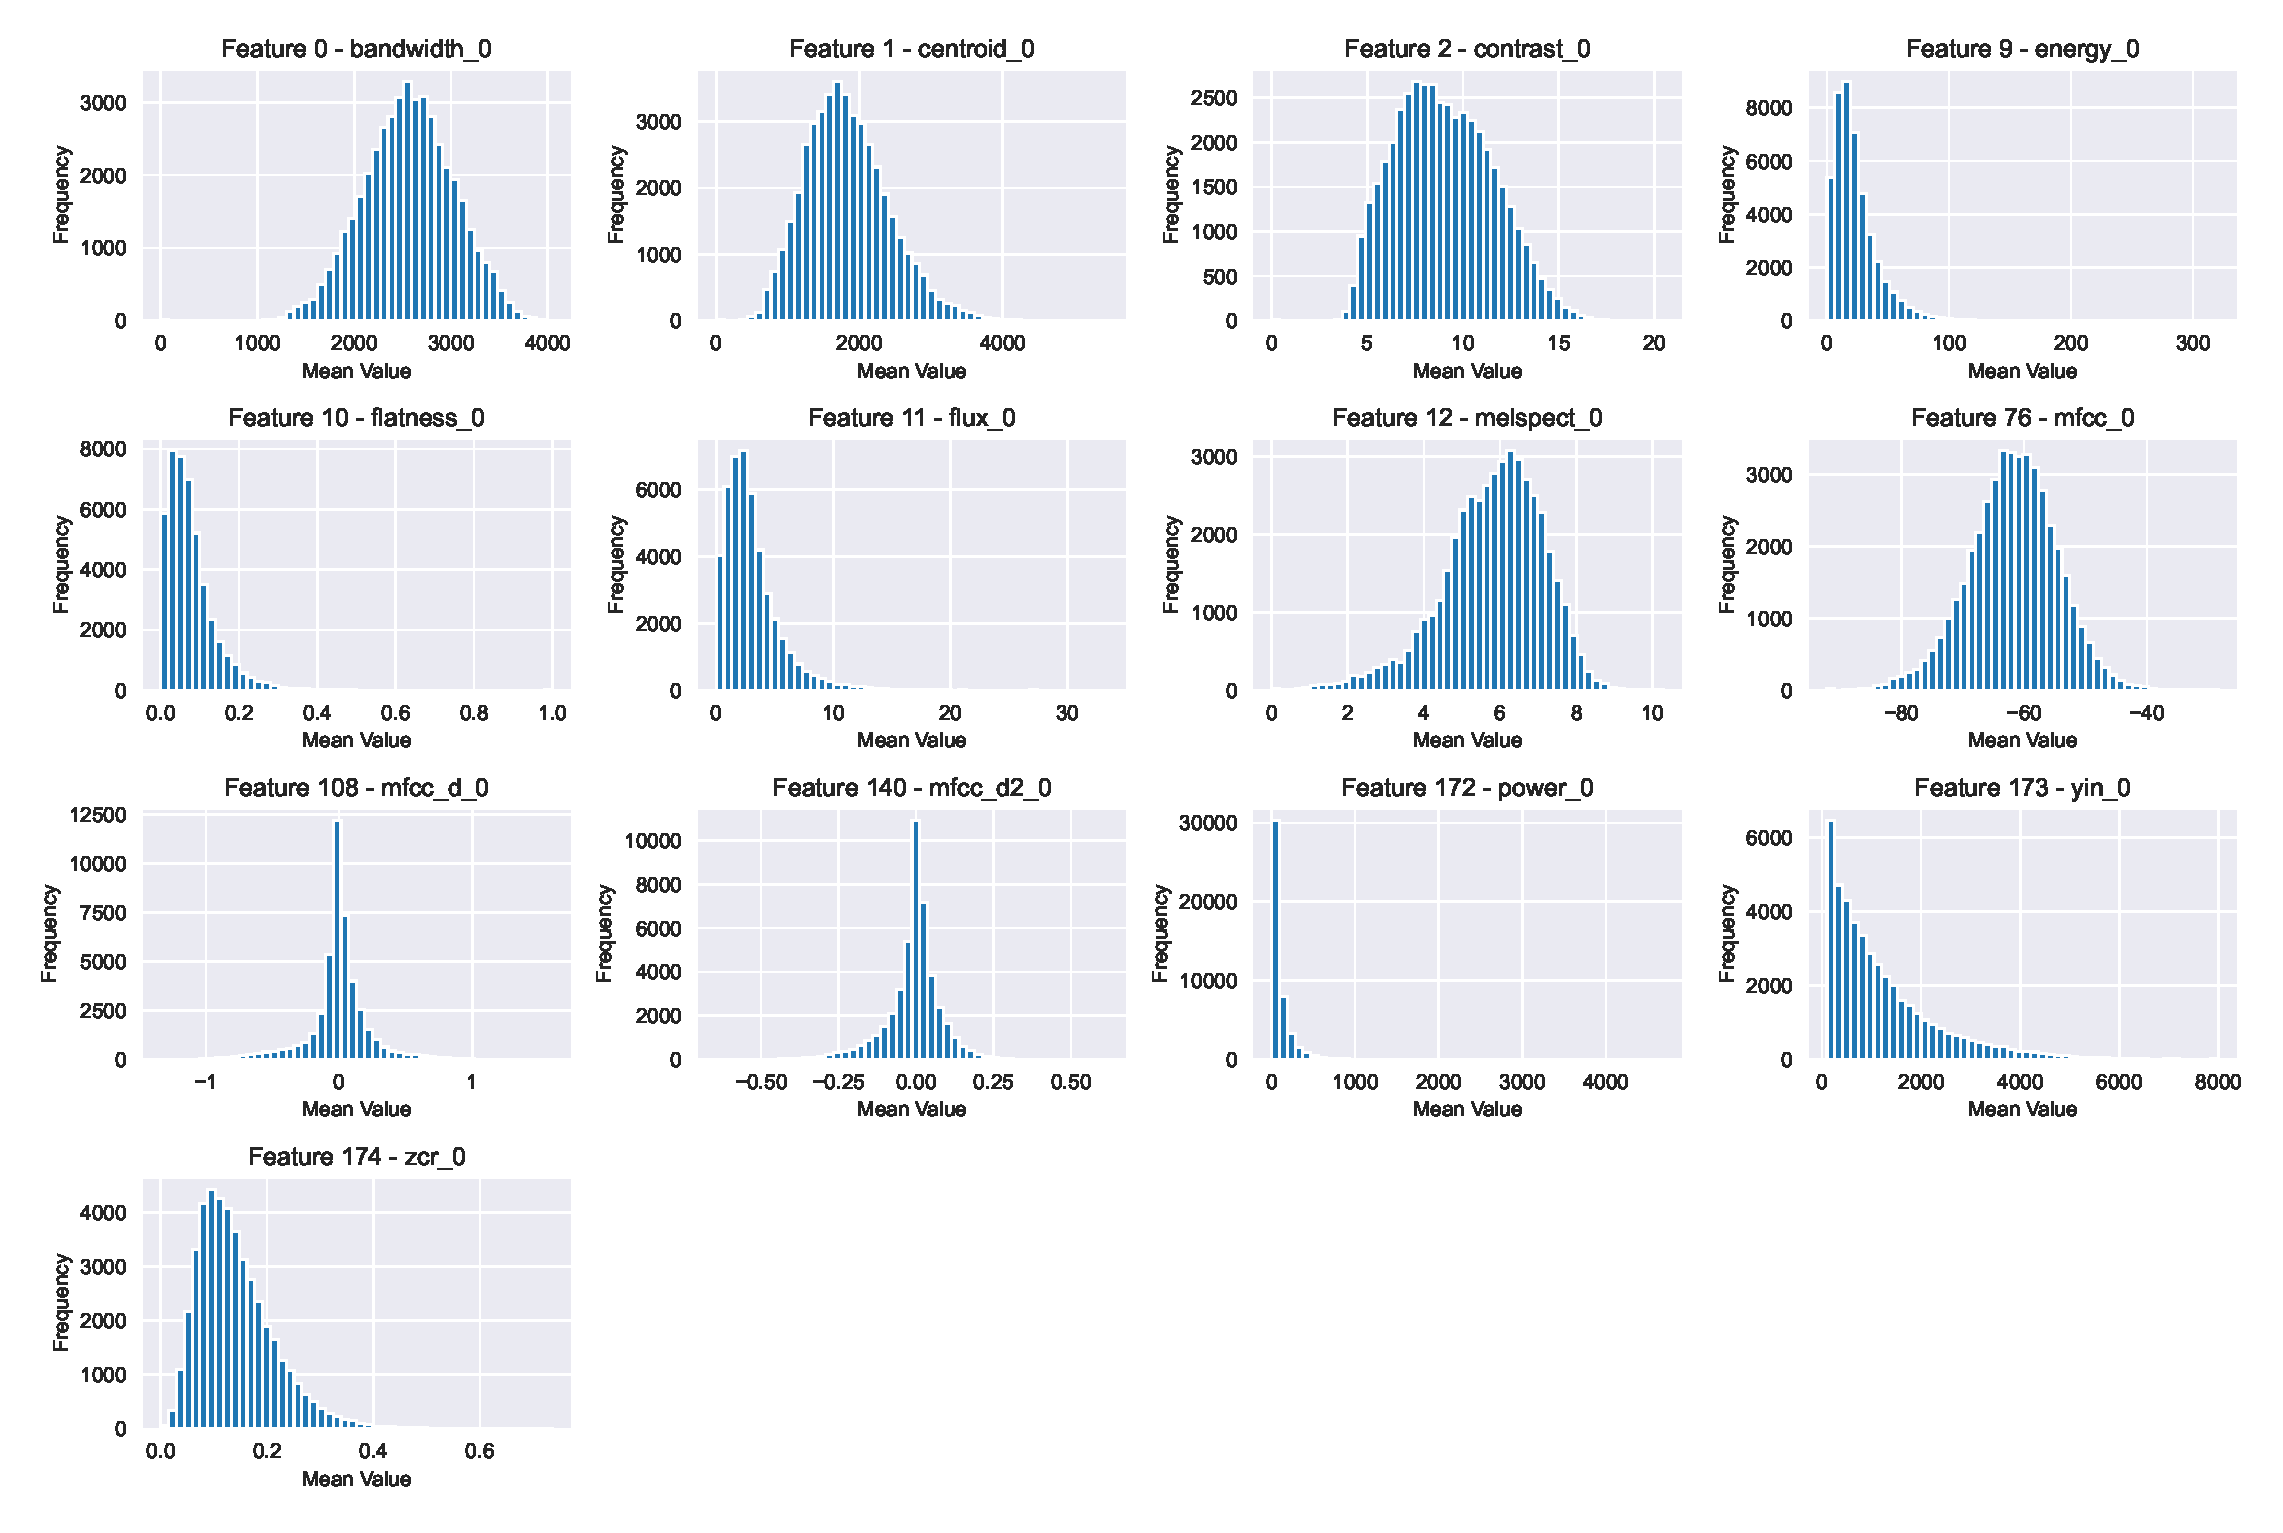
\includegraphics[scale=0.3]{fig/feature_dist}
	\vspace{-0.3cm}
	\caption{Feature Distribution.}
	\label{fig:FeatureDistribution}
	\vspace{-0.1cm}
\end{figure}


\subsection{Correlation and Redundancy}

Analyzing the correlation between features is essential to identify redundant information that could be pruned to simplify the model and reduce the risk of overfitting.

\subsubsection{Methodology:}

We applied Pearson's correlation coefficient to assess linear relationships between pairs of features. A heatmap visualization helped us quickly identify areas of high correlation, indicative of redundant information.

\subsubsection{Findings:}

\begin{itemize}
    \item \textbf{Highly Correlated Features}: Several pairs of features related to spectral properties showed high correlation (coefficients above 0.9), suggesting redundancy. For instance, mel-scaled energies, power, energy and spectral flux were often closely aligned across samples.
    \item \textbf{Redundancy Reduction}: Based on these findings, we recommend a dimensionality reduction technique, such as Principal Component Analysis (PCA), to eliminate redundant features while preserving the variance within the dataset.
\end{itemize}

\begin{figure}[!ht]
	\centering
	\begin{minipage}{0.49\textwidth}
		\centering
		\includegraphics[scale=0.3]{fig/heatmap_single}
		\caption{Correlation - All features of single frame.}
		\label{fig:HeatmapSingle}
	\end{minipage}\hfill
	\begin{minipage}{0.49\textwidth}
		\centering
		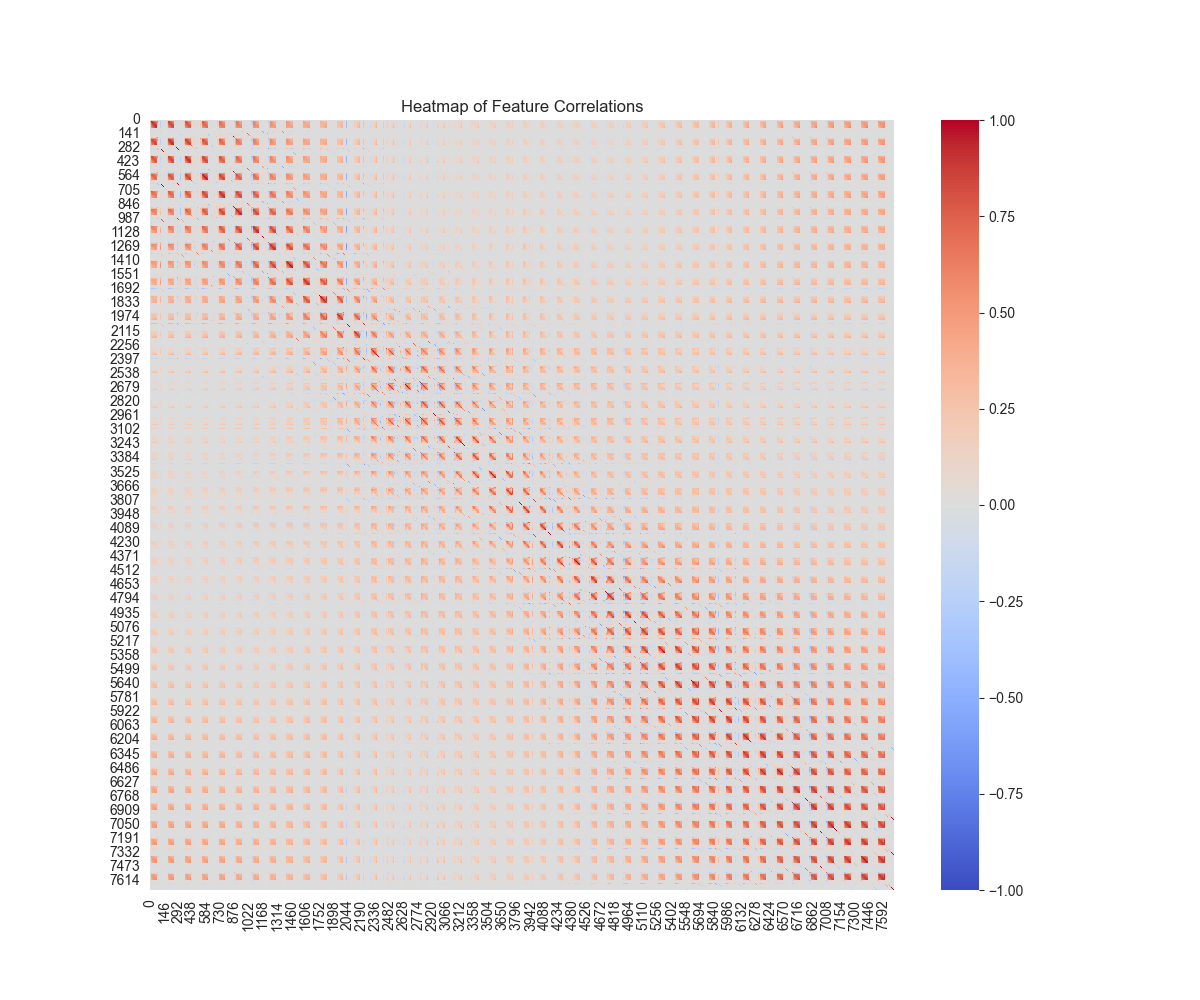
\includegraphics[scale=0.3]{fig/heatmap_all}
		\caption{Correlation - All features across all frames.}
		\label{fig:HeatmapAll}
	\end{minipage}
\end{figure}

\subsection{Speaker Variation}

Investigating whether the distribution of features varies significantly across different speakers is crucial for ensuring our model's robustness to speaker variability.

\subsubsection{Methodology:}

For this analysis, we grouped the data by speaker identity and then analyzed the variance within feature distributions across these groups.
This approach helps us to understand if and how much the speaker's identity might influence the observed feature values.

\subsubsection{Findings:}

\begin{itemize}
    \item \textbf{Variation Across Speakers}: Preliminary analysis suggests variability in certain features, particularly those related to pitch and timbre, across different speakers.
    This variability underscores the importance of including speaker normalization techniques in our preprocessing pipeline to mitigate these effects.
    \item \textbf{Normalization Techniques}: Techniques such as cepstral mean normalization (CMN)\footnote{https://en.wikipedia.org/wiki/Cepstral\textunderscore mean\textunderscore and\textunderscore variance\textunderscore normalization} or c (VAD)\footnote{https://en.wikipedia.org/wiki/Voice\textunderscore activity\textunderscore detection} could be employed to reduce the impact of speaker variability on feature distributions.
\end{itemize}

%\begin{figure}[!ht]
%	\centering
%	\begin{minipage}{0.49\textwidth}
%		\centering
%		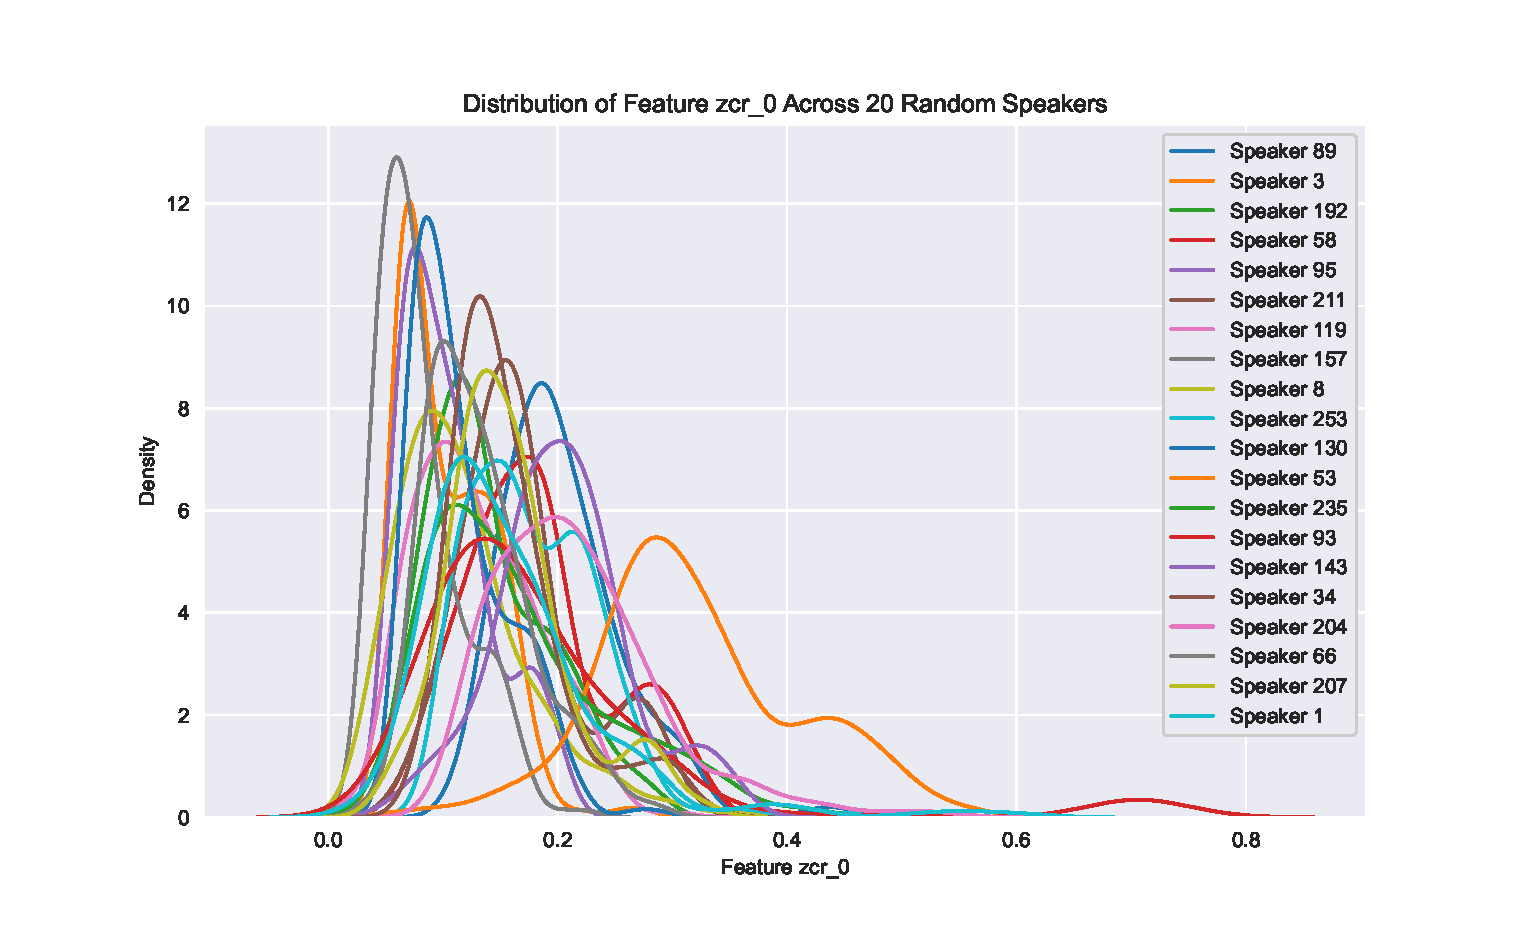
\includegraphics[scale=0.3]{fig/speakers_zcr0}
%		\caption{Speakers ZCR0}
%		\label{fig:SpeakersZcr0}
%	\end{minipage}\hfill
%	\begin{minipage}{0.49\textwidth}
%		\centering
%		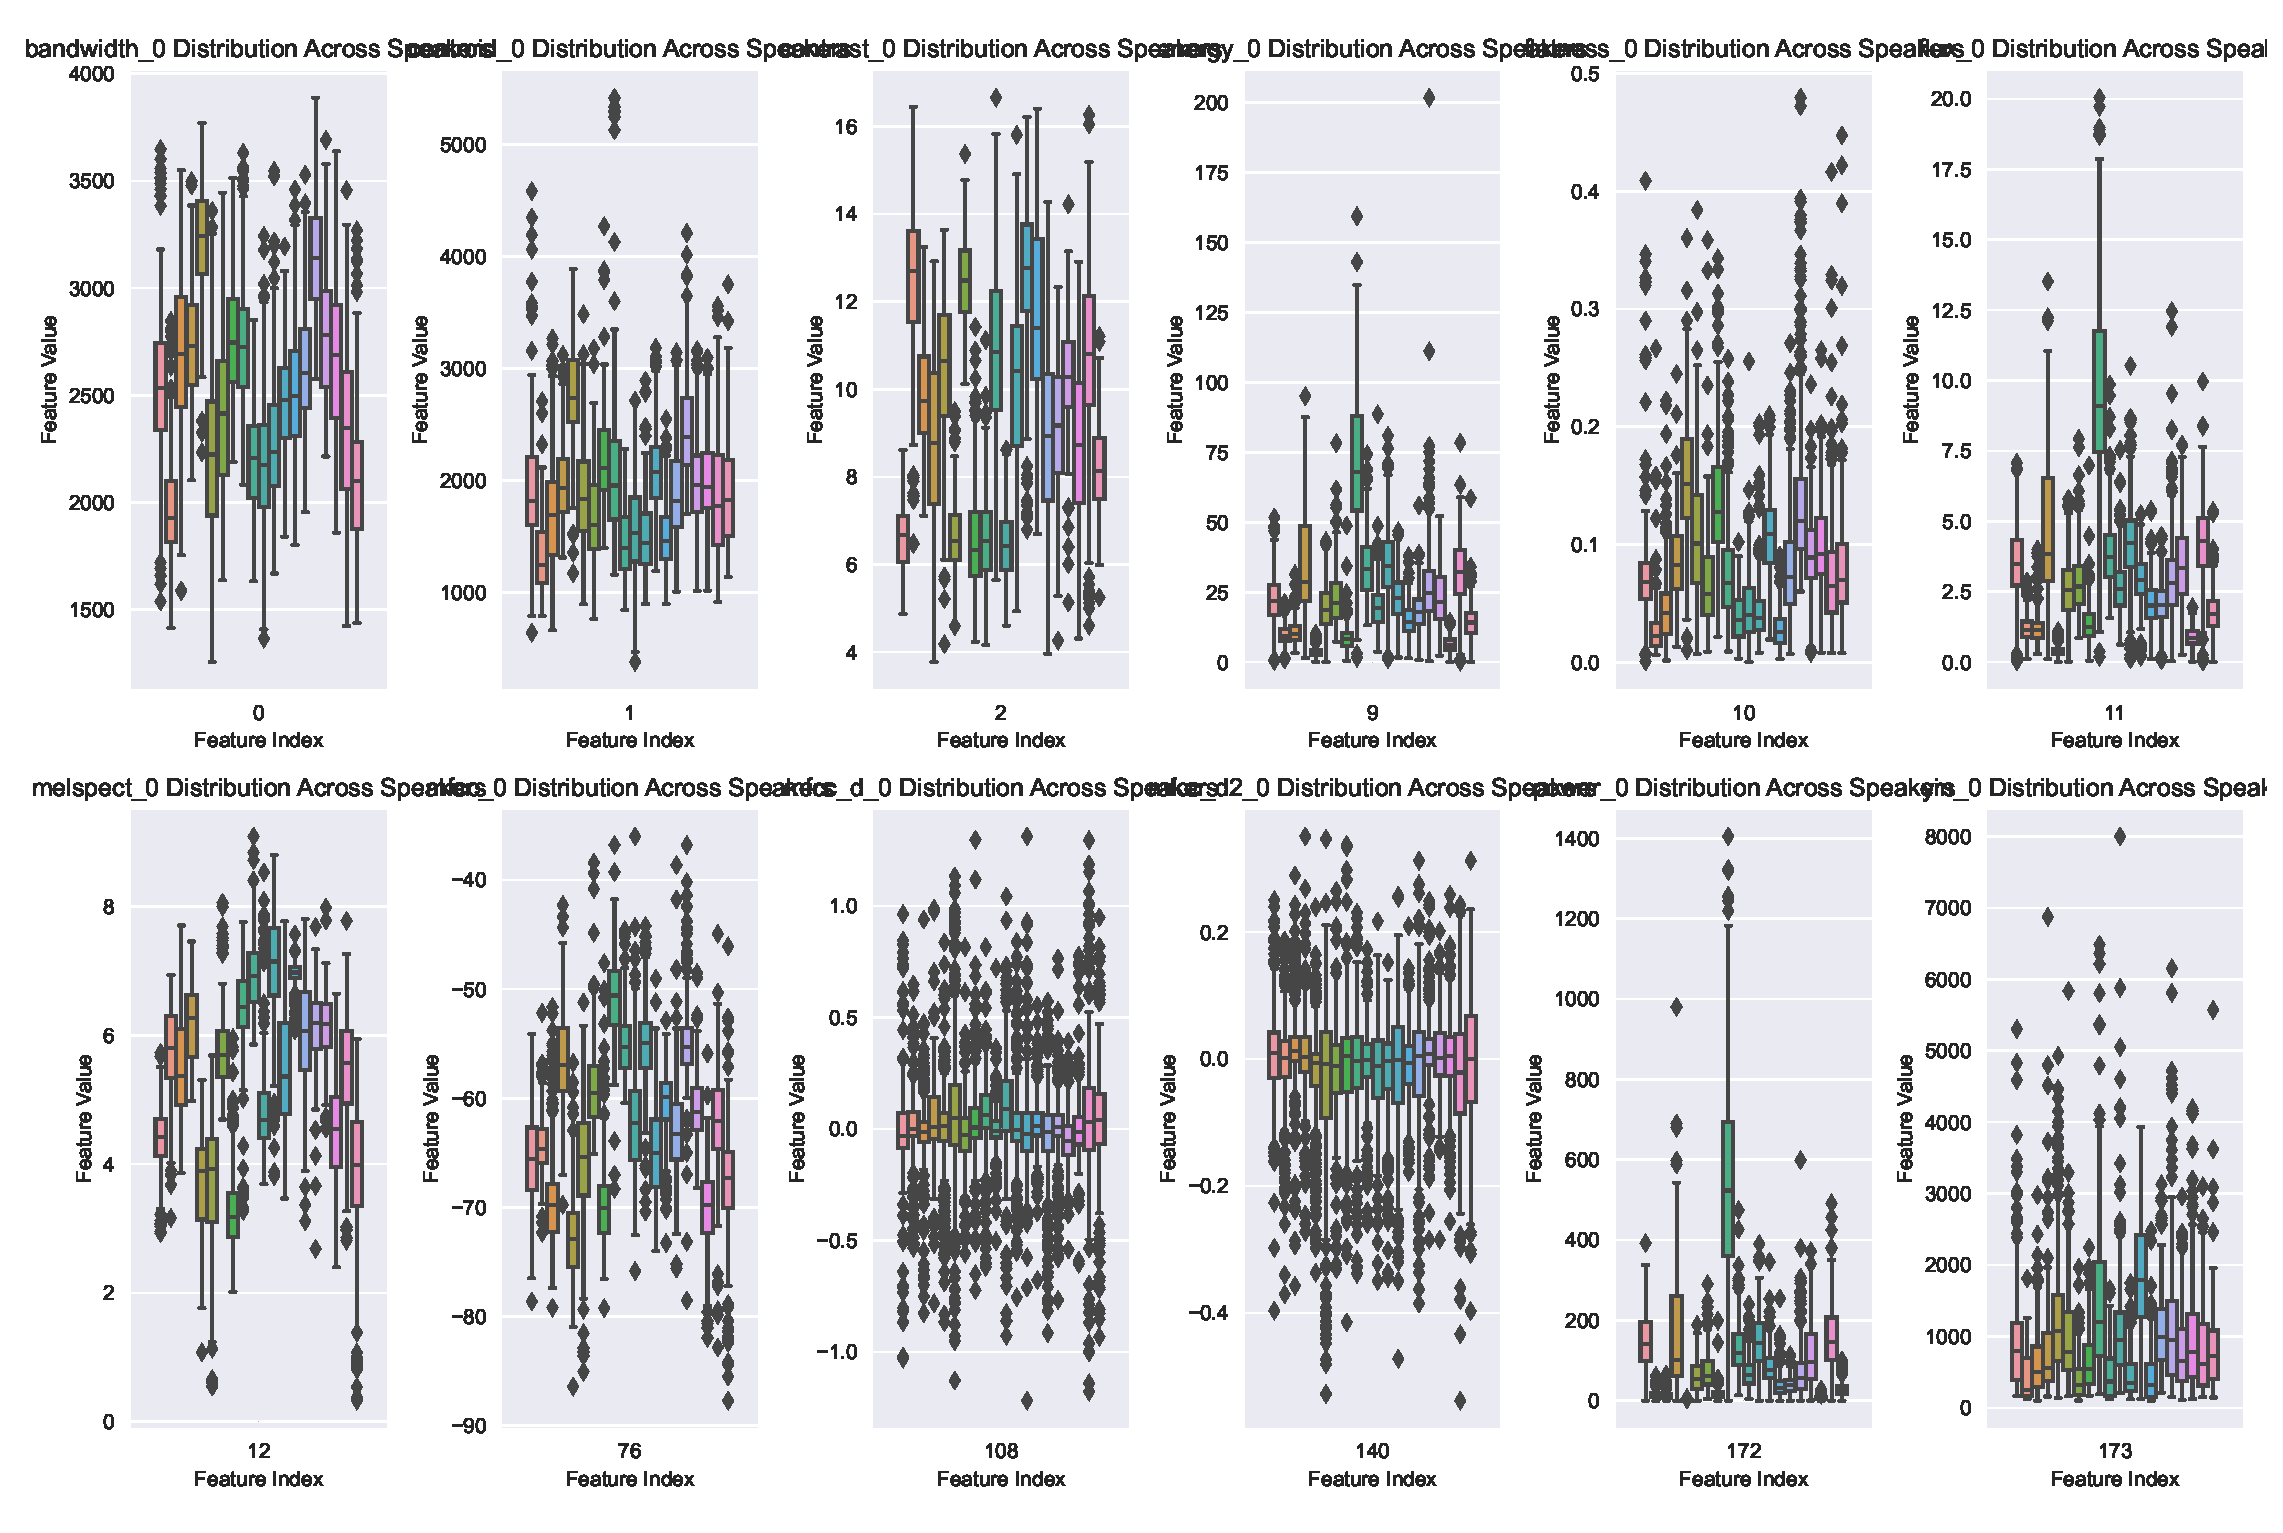
\includegraphics[scale=0.3]{fig/speakers_dist}
%		\caption{Additional Image Description.}
%		\label{fig:Speakers Dist}
%	\end{minipage}
%\end{figure}

\begin{figure}[!ht]
	\centering
	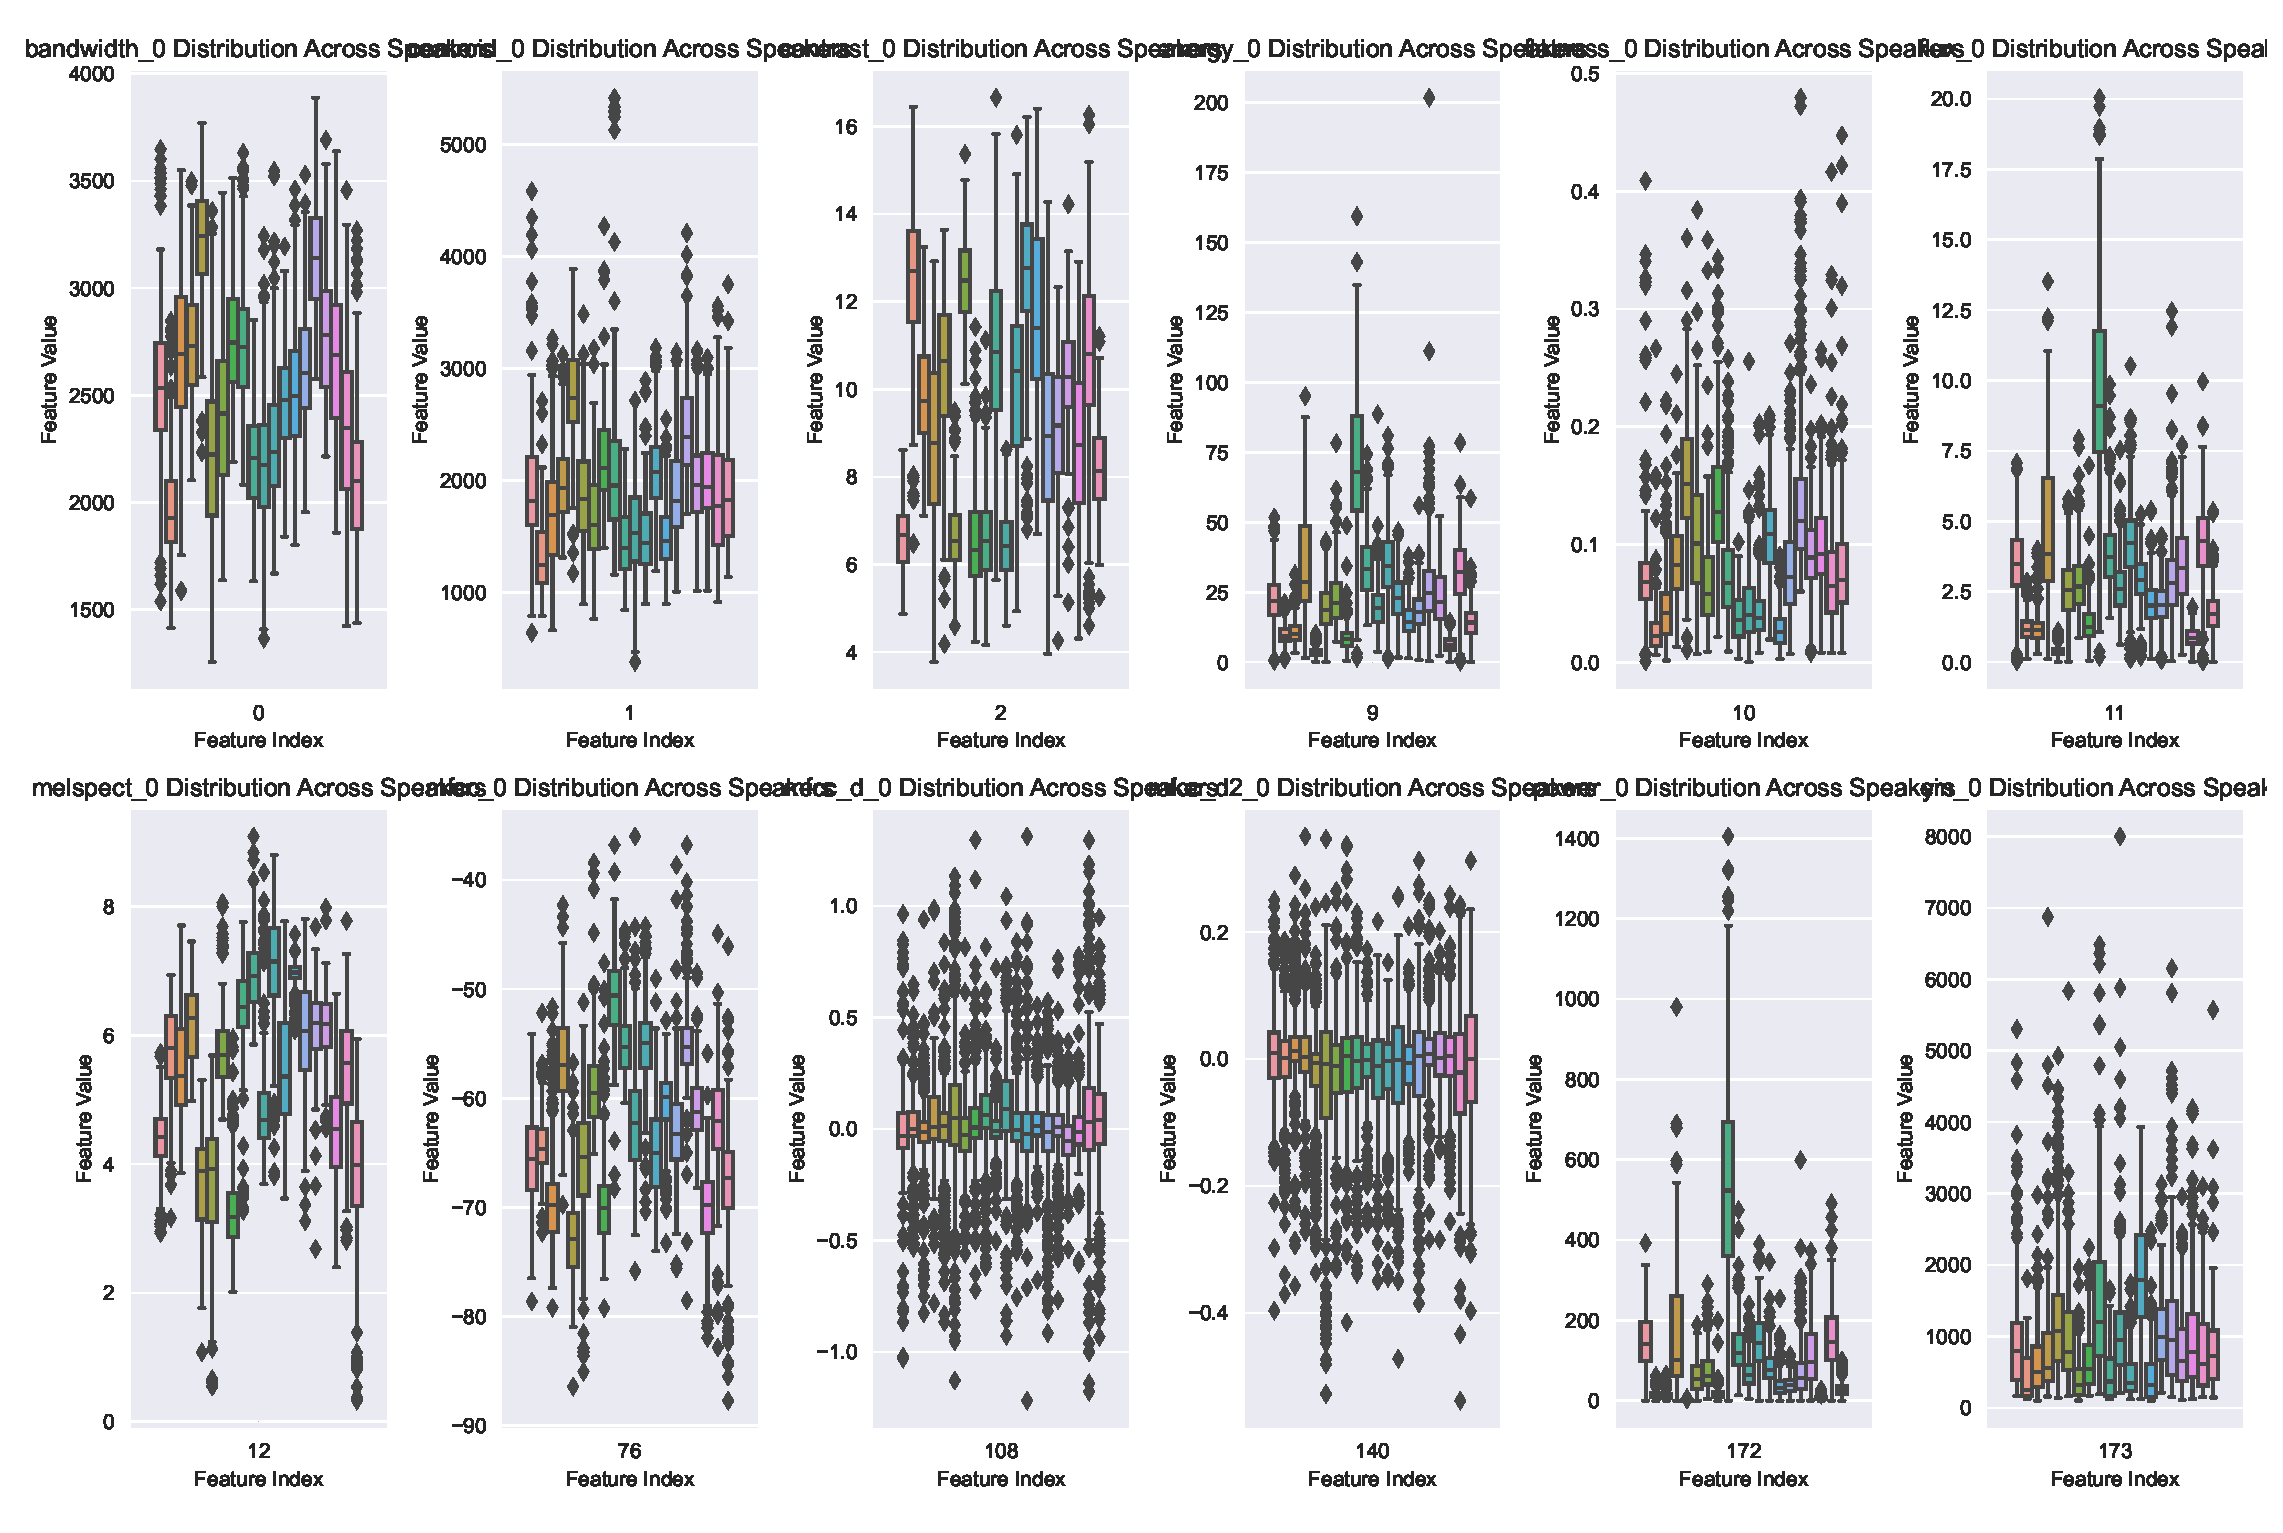
\includegraphics[scale=0.3]{fig/speakers_dist}
	\vspace{-0.3cm}
	\caption{Speakers Distribution.}
	\label{fig:SpeakersDistribution}
	\vspace{-0.1cm}
\end{figure}

\begin{figure}[!ht]
	\centering
	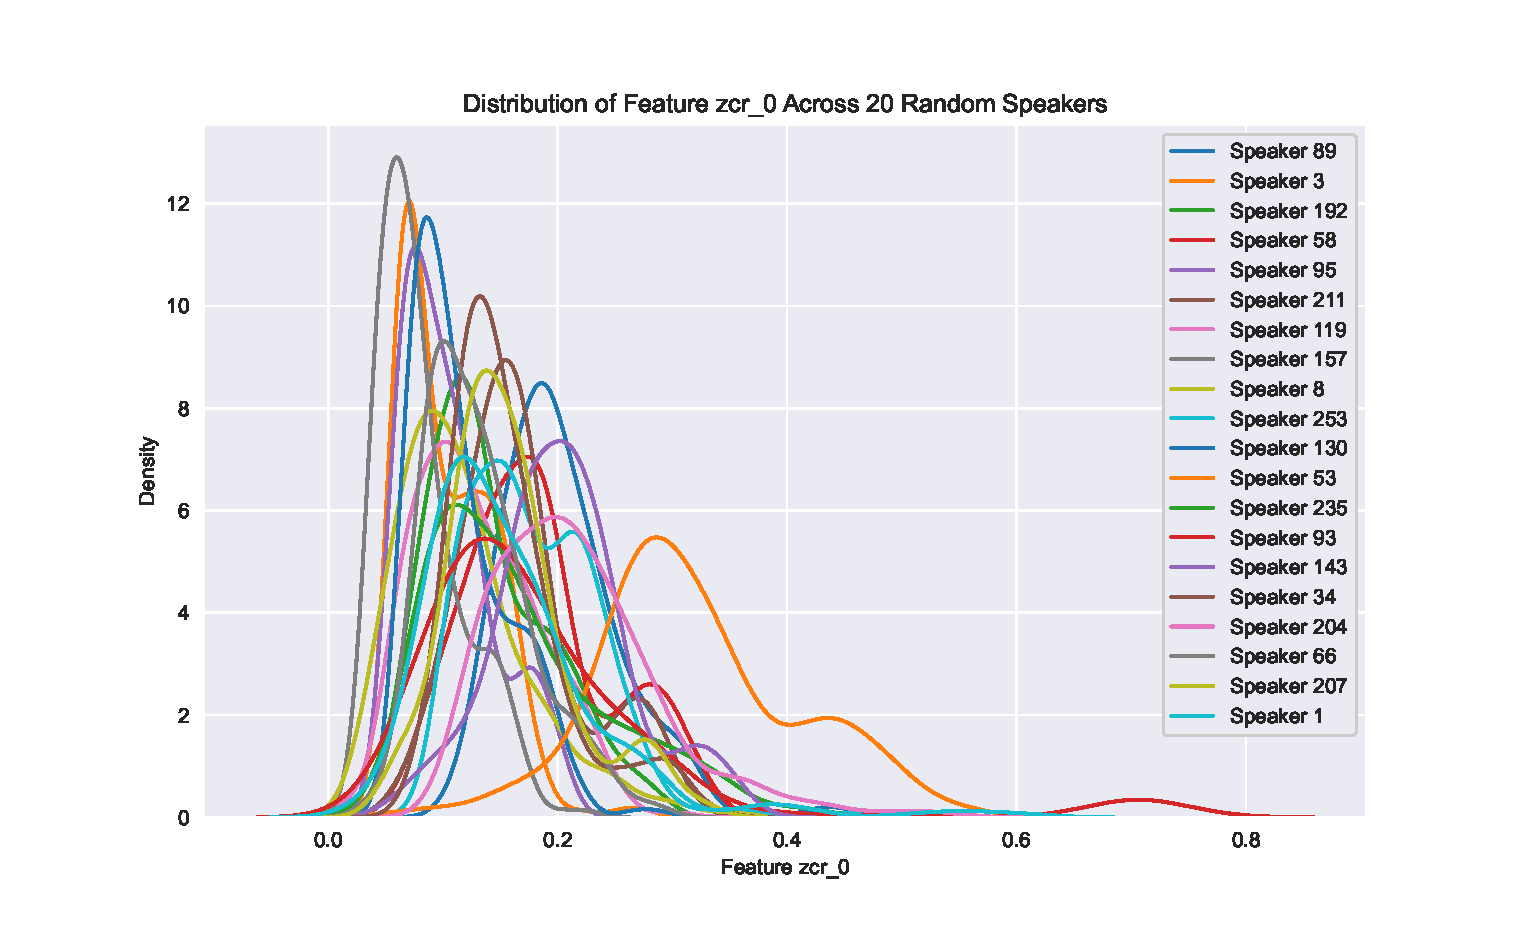
\includegraphics[scale=0.3]{fig/speakers_zcr0}
	\vspace{-0.3cm}
	\caption{Speakers ZCR0.}
	\label{fig:SpeakersZCR0}
	\vspace{-0.1cm}
\end{figure}